\subsection{The second Deformation Lemma}

\begin{theorem}[Second deformation Lemma, Milnor]
    \label{theorem:2nd deformation lemma}
    Let $M$ be a manifold, $f: M \rightarrow \R$ smooth and $p$ be a 
    non-degenerate critical point of $f$ of index $\lambda$. Let $c := f(p)$ and 
    $\varepsilon > 0$, s.th. $f^{-1}[c-\varepsilon, c+\varepsilon]$ is compact 
    and contains no critical points of $f$. Then $M^{c+\varepsilon}$ is obtained 
    from $M^{c-\varepsilon}$ by attaching a $\lambda$-cell.
 \end{theorem}
 
 \begin{proof}
    The idea of the proof is define a new function $F$, that is equal to $f$
    exept for in a small neighborhood of $p$, there we take $F < f$ slightly. 
    Then we get a situation as in the following diagram, where our manifold is
    the Torus and the map is the hight map, where $c = f(p)$:
 
    \begin{figure}[H]
       \centering
       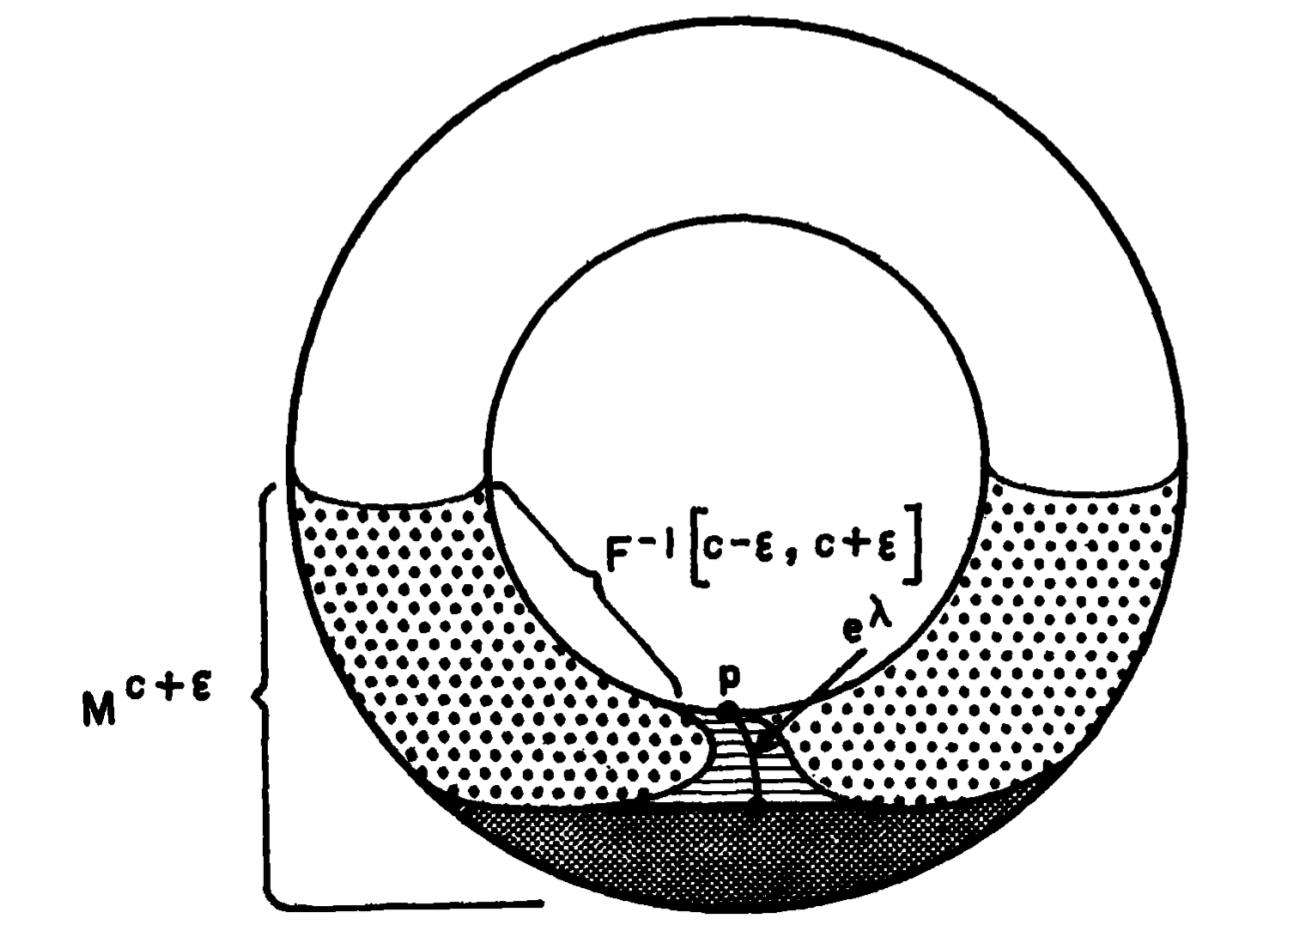
\includegraphics[width=0.5\linewidth]{resources/Mil-Diagram4.png}
       \label{fig:mil-diagram4}
    \end{figure}
 
    The heavily shaded region is $M^{c-\varepsilon}$. Then $F^{-1}(-\infty, c]$ is
    the heavily shaded region together with the horizontally shaded region. We Then
    construct a homotopy-equivalence that "squishes" the horizontally shaded region
    along the indicated lines, thus only leaving a $\lambda$-cell.
 
    By the Morse Lemma \ref{theorem:morse lemma}, we can choose local coordinates
    $\varphi = (u^1, ..., u^n)$ in a neighborhood of $p$ such that 
    \[ f = c -  (u^1)^2 - ... - (u^{\lambda})^2 + (u^{\lambda + 1})^2 + ... + (u^n)^2 \]
    in a neighborhood $U$ of $p$. Then for the critical point $p$ we have
    \[ u^1(p) = ... = u^n(p) = 0 \]
    Now choose $\varepsilon > 0$ small enough, such that the following two 
    statements hold:
    \begin{enumerate}
       \item $f^{-1}[c - \varepsilon, c + \varepsilon]$ is compact and contains
          no critical points of $f$.
       \item $\{ x: \lVert x \rVert \leq 2\varepsilon \} \subseteq \varphi(U)$
    \end{enumerate}
 
    Now choose the $\lambda$-cell $e^{\lambda}$ to be the points in M with
    \[ (u^1)^2 + ... + (u^{\lambda})^2 \leq \varepsilon 
    \text{ and } u^{\lambda + 1} = ... = u^n = 0 \].
 
    We now have our mainfold parametrized in $U$ in a nice way. The situation is
    illustrated in the following diagram:
 
    \begin{figure}[H]
       \centering
       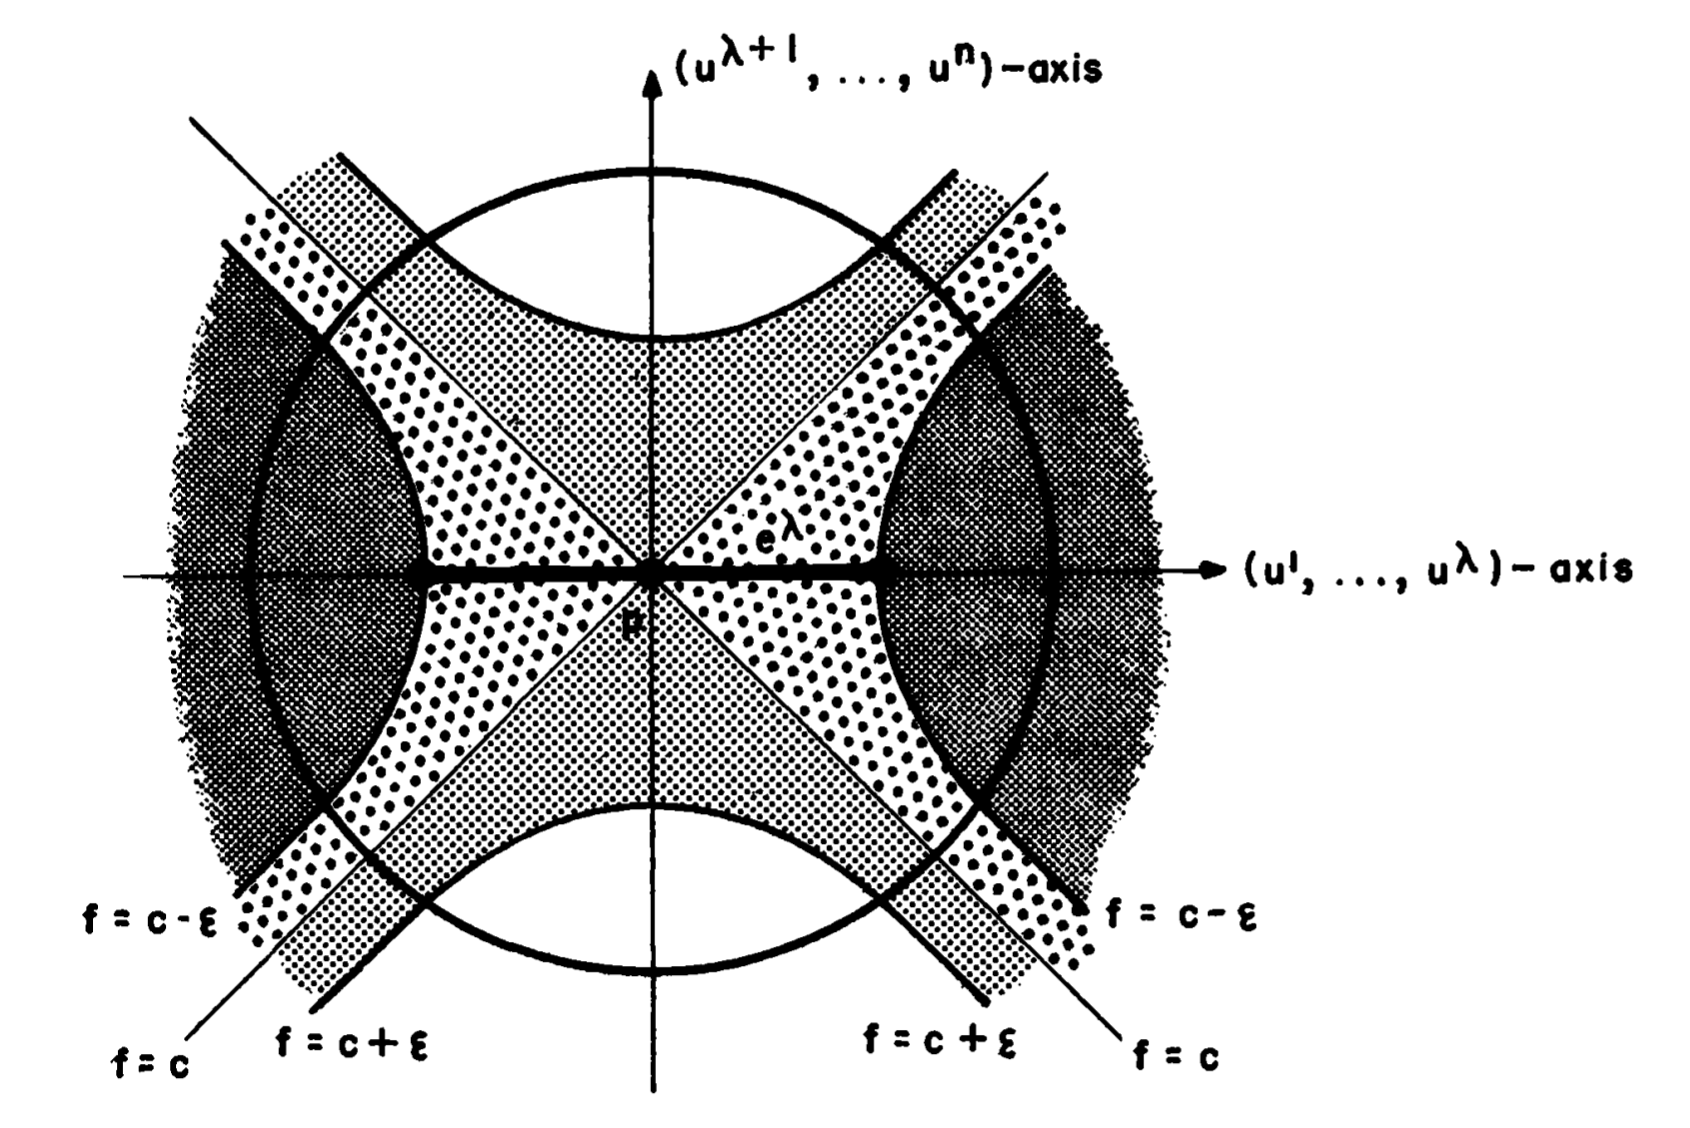
\includegraphics[width=0.7\linewidth]{resources/Mil-Diagram5.png}
       \label{fig:mil-diagram5}
    \end{figure}
 
    The heavily shaded area is $M^{c-\varepsilon}$, the area shaded with bigger
    dots is $f^{-1}[c - \varepsilon, c]$ and the area shaded with smaller dots
    is $f^{-1}[c, c + \varepsilon]$. \\
    The circle is $\{ p \in M : u^1(p) + ... + u^n(p) = \sqrt{2\varepsilon} \}$.
    Notice that $e^\lambda \cap M^{c - \varepsilon} = \partial e^{\lambda}$, so
    it is atteched to $M^{c - \varepsilon}$ as required. We now have to show that
    $e^{\lambda} \cup M^{c - \varepsilon}$ is a deformation retract of 
    $M^{c + \varepsilon}$. \\
    Define a $C^{\infty}$ function $\mu : \R \rightarrow \R$ with the following
    properties:
    \begin{align*}
       & \mu(0) > \varepsilon \\
       & \mu(r) = 0 \text{ for } r \geq 2\varepsilon \\
       & -1 < \mu'(r) \leq 0 \text{ for all } r
    \end{align*}
 
    Now let $F$ equal $f$ outside of $U$, and let 
    \[ F = f - \mu((u^1)^2 + ... + (u^{\lambda})^2 + 2(u^{\lambda + 1})^2 + ... + 2(u^n)^2) \]
    within $U$. $F$ is well defined and smooth, because for 
    $ ((u^1)^2 + ... + (u^n)^2)(p) > 2\varepsilon $, $\mu(p) = 0$ and the closed
    ball with radius $\sqrt{2\varepsilon}$ is fully contained in $U$. \\
    Now define 
    \[ \xi, \eta: U \rightarrow [0, \infty) \]
    by
    \begin{align*}
       & \xi = (u^1)^2 + ... + (u^n)^2 \\
       & \eta = (u^{\lambda + 1})^2 + ... + (u^n)^2
    \end{align*}
    Then $f = c - \xi + \eta$ and $F|_U = f - \mu(\xi + 2\eta) = c - \xi + \eta - \mu(\xi + 2\eta)$
 
    Assertion 1: The region $F^{-1}(-\infty, c + \varepsilon]$ coincides with 
    $M^{c + \varepsilon}$.
 
    For $\xi(p) + 2 \eta(p) > 2 \varepsilon$, $f(p) = F(p)$. So wlog., 
    let $p \in M$ such that $\xi(p) + 2 \eta(p) \leq 2 \varepsilon$. Then 
    \[ F(p) \leq f(p) = c + \xi(p) + \eta(p) 
    \leq c + \frac{1}{2} \xi(p) + \eta(p) 
    \leq c + \varepsilon \]. 
    This prooves the first assertion.
 
    Assertion 2: The critical points of $F$ are the same as those of $f$.
 
    Note that 
    \[ \pderive[F]{\xi} = -1 - \mu'(\xi + 2 \eta) < 0\]
    and
    \[ \pderive[F]{\eta} = 1 - 2 \mu'(\xi + 2 \eta) \geq 1 \]
    , so in particular these derivatives are never $0$. Since 
    \[ \text{d}F = \pderive[F]{\xi}\text{d}\xi + \pderive[F]{\eta} \text{d}\eta \]
    And d$\xi$ and d$\eta$ are zero only in $p$, $F$ has no critical points
    in $U$ other then $p$. This proves the second assertion.
 
    Assertion 3: The region $F^{-1}(-\infty, c - \varepsilon]$ is a deformation 
    retract of $M^{c + \varepsilon}$.
 
    Consider the region $F^{-1}[c - \varepsilon, c + \varepsilon]$. With 
    assertion 1 and the fact that $F \leq f$, we see that
    \[ F^{-1}[c - \varepsilon, c + \varepsilon] \subseteq f^{-1}[c - \varepsilon, c + \varepsilon] \] .
    But $f^{-1}[c - \varepsilon, c + \varepsilon]$ is compact and 
    $F^{-1}[c - \varepsilon, c + \varepsilon]$ is closed, so it is compact as 
    well. By assertion 2, it cannot contain any critical points of $F$ exept 
    maybe $p$, but
    \[ F(p) = c - \mu(0) < c - \varepsilon \],
    so $p$ is not in the region. Then with the first deformation 
    lemma~\ref{theorem:1st deformation lemma}, the third assertion is proven.
    
    In the following, $H$ will be the closure of 
    $F^{-1}(- \infty, c - \varepsilon] - M^{c - \varepsilon}$, which we shall call
    a "handle". So $F^{-1}(- \infty, c - \varepsilon] = M^{c - \varepsilon} \cup H$
    will be called "$M^{c - \varepsilon}$ with a handle attached".

    Now consider $e^{\lambda}$ from above, i.e. the $\lambda$-cell consisting of
    all points $q$ with
    \[ \xi(q) \leq \varepsilon \text{ and } \eta(q) = 0 \].
    Note that $e^{\lambda}$ is contained in the handle $H$. In fact, since 
    $\pderive[F]{\xi} < 0$, we have
    \[ F(q) \leq F(p) < c - \varepsilon \],
    but $f(q) \geq c - \varepsilon$ for $q \in e^{\lambda}$.
    
    %TODO
    \textbf{TODO}
 \end{proof}